
%(BEGIN_QUESTION)
% Copyright 2010, Tony R. Kuphaldt, released under the Creative Commons Attribution License (v 1.0)
% This means you may do almost anything with this work of mine, so long as you give me proper credit

Et DDC-system for byggautomasjon sender 4-20 mA styresignal til en dampventil med elektronisk posisjoner. Sløyfen har et problem: ventilen står helt stengt (0\%) uansett hva DDC forsøker å gjøre. En tekniker starter feilsøkingen med DC-spenningsmåling på klemrekke TB-11:

$$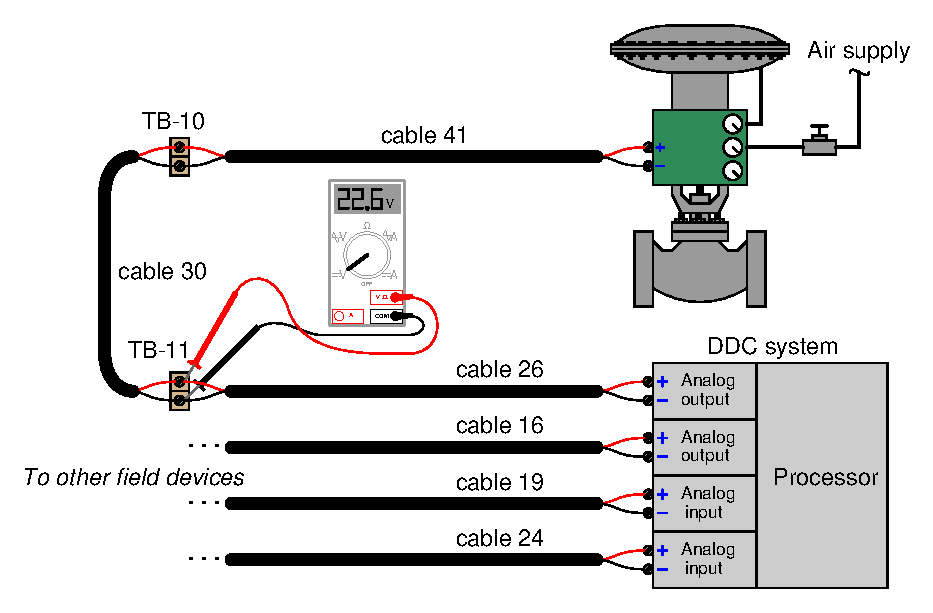
\includegraphics[width=15.5cm]{i00717x01.eps}$$

Teknikeren vet at 22.6 volt tilsvarer "åpen" feil. Ut fra målepunkt og målt verdi (22.6 VDC), bestem hvor i ledningsnettet en enkelt åpen feil kan være.

\vskip 10pt

Deretter kobler teknikeren en midlertidig jumper over TB-10 mens målingen på TB-11 fortsetter. Ny måling blir 0.0 volt. Hva forteller dette om feiltype og feilsted?

\vskip 10pt

Forklar om det er fare for kortslutning ved denne testen. Kan en sikring ryke?

\vskip 20pt \vbox{\hrule \hbox{\strut \vrule{} {\bf Forslag til sokratisk diskusjon} \vrule} \hrule}

\begin{itemize}
\item{} Forklar hvorfor det er kritisk å vite om ventil og DDC-kort er elektriske {\it kilder} eller {\it laster} når spenningsmålinger tolkes.
\item{} Beskriv fordeler/ulemper med denne teststilen (måle før/etter bevisst kortslutning) sammenlignet med andre multimetertester for å finne åpen feil.
\item{} Beskriv en god "neste test" for å avgrense feiltype og lokasjon ytterligere.
\end{itemize}

\underbar{file i00717no}
%(END_QUESTION)





%(BEGIN_ANSWER)


%(END_ANSWER)





%(BEGIN_NOTES)

Basert på første måling alene kan feilen {\it være} åpen feil enten i kabel 30 eller i kabel 41.

\vskip 10pt

Etter andre måling må vi konkludere med åpen feil i kabel 41 (eller åpen feil i ventilposisjoneren).

\vskip 10pt

Det er ingen fare ved å introdusere en kortslutning her, fordi DDC-kortets 4-20 mA-utgang er naturlig strømbegrenset som andre 4-20 mA-utganger.

%INDEX% Feilsøking, repetisjon: elektriske kretser

%(END_NOTES)
